% Options for packages loaded elsewhere
\PassOptionsToPackage{unicode}{hyperref}
\PassOptionsToPackage{hyphens}{url}
%
\documentclass[
]{article}
\usepackage{amsmath,amssymb}
\usepackage{iftex}
\ifPDFTeX
  \usepackage[T1]{fontenc}
  \usepackage[utf8]{inputenc}
  \usepackage{textcomp} % provide euro and other symbols
\else % if luatex or xetex
  \usepackage{unicode-math} % this also loads fontspec
  \defaultfontfeatures{Scale=MatchLowercase}
  \defaultfontfeatures[\rmfamily]{Ligatures=TeX,Scale=1}
\fi
\usepackage{lmodern}
\ifPDFTeX\else
  % xetex/luatex font selection
\fi
% Use upquote if available, for straight quotes in verbatim environments
\IfFileExists{upquote.sty}{\usepackage{upquote}}{}
\IfFileExists{microtype.sty}{% use microtype if available
  \usepackage[]{microtype}
  \UseMicrotypeSet[protrusion]{basicmath} % disable protrusion for tt fonts
}{}
\makeatletter
\@ifundefined{KOMAClassName}{% if non-KOMA class
  \IfFileExists{parskip.sty}{%
    \usepackage{parskip}
  }{% else
    \setlength{\parindent}{0pt}
    \setlength{\parskip}{6pt plus 2pt minus 1pt}}
}{% if KOMA class
  \KOMAoptions{parskip=half}}
\makeatother
\usepackage{xcolor}
\usepackage[margin=1in]{geometry}
\usepackage{longtable,booktabs,array}
\usepackage{calc} % for calculating minipage widths
% Correct order of tables after \paragraph or \subparagraph
\usepackage{etoolbox}
\makeatletter
\patchcmd\longtable{\par}{\if@noskipsec\mbox{}\fi\par}{}{}
\makeatother
% Allow footnotes in longtable head/foot
\IfFileExists{footnotehyper.sty}{\usepackage{footnotehyper}}{\usepackage{footnote}}
\makesavenoteenv{longtable}
\usepackage{graphicx}
\makeatletter
\def\maxwidth{\ifdim\Gin@nat@width>\linewidth\linewidth\else\Gin@nat@width\fi}
\def\maxheight{\ifdim\Gin@nat@height>\textheight\textheight\else\Gin@nat@height\fi}
\makeatother
% Scale images if necessary, so that they will not overflow the page
% margins by default, and it is still possible to overwrite the defaults
% using explicit options in \includegraphics[width, height, ...]{}
\setkeys{Gin}{width=\maxwidth,height=\maxheight,keepaspectratio}
% Set default figure placement to htbp
\makeatletter
\def\fps@figure{htbp}
\makeatother
\setlength{\emergencystretch}{3em} % prevent overfull lines
\providecommand{\tightlist}{%
  \setlength{\itemsep}{0pt}\setlength{\parskip}{0pt}}
\setcounter{secnumdepth}{-\maxdimen} % remove section numbering
\usepackage{booktabs}
\usepackage{longtable}
\usepackage{array}
\usepackage{multirow}
\usepackage{wrapfig}
\usepackage{float}
\usepackage{colortbl}
\usepackage{pdflscape}
\usepackage{tabu}
\usepackage{threeparttable}
\usepackage{threeparttablex}
\usepackage[normalem]{ulem}
\usepackage{makecell}
\usepackage{xcolor}
\ifLuaTeX
  \usepackage{selnolig}  % disable illegal ligatures
\fi
\usepackage{bookmark}
\IfFileExists{xurl.sty}{\usepackage{xurl}}{} % add URL line breaks if available
\urlstyle{same}
\hypersetup{
  pdftitle={UNICEF Coverage Report: Antenatal Care and Skilled Birth Attendance (2018--2022)},
  pdfauthor={UNICEF D\&A Education Team},
  hidelinks,
  pdfcreator={LaTeX via pandoc}}

\title{UNICEF Coverage Report: Antenatal Care and Skilled Birth
Attendance (2018--2022)}
\author{UNICEF D\&A Education Team}
\date{}

\begin{document}
\maketitle

\begin{quote}
\textbf{About this Submission}\\
This technical report supports the application to the following UNICEF
D\&A consultancy positions:\\
-- Learning and Skills Data Analyst Consultant (\#581598)\\
-- Household Survey Data Analyst Consultant (\#581656)\\
-- Administrative Data Analyst Consultant (\#581696)\\
-- Microdata Harmonization Consultant (\#581699)
\end{quote}

\section{1. Context, Objectives and
Methodology}\label{context-objectives-and-methodology}

\begin{center}\rule{0.5\linewidth}{0.5pt}\end{center}

\begin{quote}
\textbf{About this Report}\\
This technical note summarizes coverage of maternal health services
across UNICEF-focus countries. Countries are classified as
\textbf{on-track} or \textbf{off-track} based on under-five mortality
status (U5MR), aligned with \textbf{SDG 3.2}. The indicators analyzed
--- ANC4 and SBA --- are key components of the maternal care continuum
and contribute to the achievement of \textbf{SDG 3.1}.
\end{quote}

\begin{center}\rule{0.5\linewidth}{0.5pt}\end{center}

\subsubsection{Context}\label{context}

Reducing \textbf{under-five mortality} remains a global priority ---
particularly in countries where maternal health services are limited or
inequitable. To assess readiness and identify service gaps, UNICEF
monitors two critical indicators of maternal care:

\begin{itemize}
\tightlist
\item
  \textbf{ANC4}: Percentage of women (aged 15--49) receiving at least
  \textbf{four antenatal care visits}.
\item
  \textbf{SBA}: Percentage of births attended by \textbf{skilled health
  personnel}.
\end{itemize}

These indicators reflect \textbf{early engagement} in pregnancy and
\textbf{safe delivery}, both essential to reducing maternal and neonatal
mortality. Together, they form a core part of the continuum of care.

To contextualize coverage performance, countries are grouped using the
latest \textbf{under-five mortality rate (U5MR) classification}:

\begin{itemize}
\tightlist
\item
  \textbf{On-track}: U5MR is \emph{achieved} or \emph{on-track} to meet
  \textbf{SDG target 3.2}.
\item
  \textbf{Off-track}: U5MR status is \emph{acceleration needed}.
\end{itemize}

This classification provides a framework to assess how service coverage
aligns with child survival progress and helps inform areas where
additional attention may be needed to meet \textbf{SDG target 3.2} on
ending preventable child deaths.

\begin{center}\rule{0.5\linewidth}{0.5pt}\end{center}

\subsubsection{Methodology}\label{methodology}

\paragraph{1. Data Preparation}\label{data-preparation}

\begin{itemize}
\tightlist
\item
  \textbf{ANC4} and \textbf{SBA} coverage data were retrieved from the\\
  \href{https://data.unicef.org/resources/data_explorer/unicef_f/?ag=UNICEF&df=GLOBAL_DATAFLOW&ver=1.0&dq=.MNCH_ANC4+MNCH_SAB.&startPeriod=2018&endPeriod=2022}{UNICEF
  Global Data Repository}\\
  for all available countries between \textbf{2018 and 2022}.
\item
  For each country, the \textbf{most recent coverage estimate} within
  this period was retained.
\item
  \textbf{Under-five mortality classification} (on-track / off-track)
  was assigned using the\\
  file \texttt{On-track\ and\ off-track\ countries.xlsx}, based on U5MR
  status:

  \begin{itemize}
  \tightlist
  \item
    \emph{On-track} = ``achieved'' or ``on-track''
  \item
    \emph{Off-track} = ``acceleration needed''
  \end{itemize}
\item
  All datasets were merged using standardized \textbf{ISO3 country
  codes}.
\end{itemize}

\paragraph{2. Population-Weighted
Averages}\label{population-weighted-averages}

\begin{itemize}
\tightlist
\item
  \textbf{Birth projections for 2022} were sourced from the UN World
  Population Prospects:\\
  \texttt{WPP2022\_GEN\_F01\_DEMOGRAPHIC\_INDICATORS\_COMPACT\_REV1.xlsx}.
\item
  For each group (on-track and off-track), \textbf{weighted means} were
  computed for ANC4 and SBA using birth counts as weights.
\item
  Countries with missing coverage data were excluded from group-level
  weighted statistics.
\end{itemize}

\begin{center}\rule{0.5\linewidth}{0.5pt}\end{center}

\begin{quote}
\textbf{Data Sources and Limitations}\\
- \textbf{Date of extraction and processing}: July 2025\\
- \textbf{Inputs}:\\
- ANC4 and SBA indicators from the
\href{https://data.unicef.org/resources/data_explorer/unicef_f/?ag=UNICEF&df=GLOBAL_DATAFLOW&ver=1.0&dq=.MNCH_ANC4+MNCH_SAB.&startPeriod=2018&endPeriod=2022}{UNICEF
Global Data Repository}\\
- Birth projections from the \emph{UN World Population Prospects 2022}\\
- U5MR groupings from UNICEF's official classification

Several countries were \textbf{excluded or only partially included} due
to missing data (e.g., births, U5MR status, ANC4 or SBA coverage).\\
These limitations were accounted for in the weighted analysis and are
examined in detail in \textbf{Section 2.2 on data completeness}.
\end{quote}

\begin{center}\rule{0.5\linewidth}{0.5pt}\end{center}

\section{2. Analysis of Coverage and
Gaps}\label{analysis-of-coverage-and-gaps}

This section presents group-level and country-level results for ANC4 and
SBA coverage, highlighting disparities, data quality issues, and
patterns relevant for maternal health programming.

\begin{center}\rule{0.5\linewidth}{0.5pt}\end{center}

\subsubsection{2.1 Summary coverage statistics by
group}\label{summary-coverage-statistics-by-group}

\begin{longtable}[t]{lrrrrr}
\caption{\label{tab:unnamed-chunk-1}Coverage Summary by Group}\\
\toprule
Group & \# Countries & Avg. ANC4 & Avg. SBA & Missing ANC4 & Missing SBA\\
\midrule
off-track & 46 & 61.3 & 76.3 & 4 & 2\\
on-track & 102 & 85.4 & 97.9 & 62 & 1\\
\bottomrule
\end{longtable}

\textbf{Interpretation}\\
This table shows the average ANC4 and SBA coverage for on-track and
off-track countries, along with the number of countries and missing
values.

Key insights include: - SBA coverage is consistently high across both
groups. - ANC4 coverage is lower and more variable, especially in
off-track countries. - Over 60\% of on-track countries have no ANC4
data, limiting comparability.

\begin{center}\rule{0.5\linewidth}{0.5pt}\end{center}

\subsubsection{2.2 Data completeness by
indicator}\label{data-completeness-by-indicator}

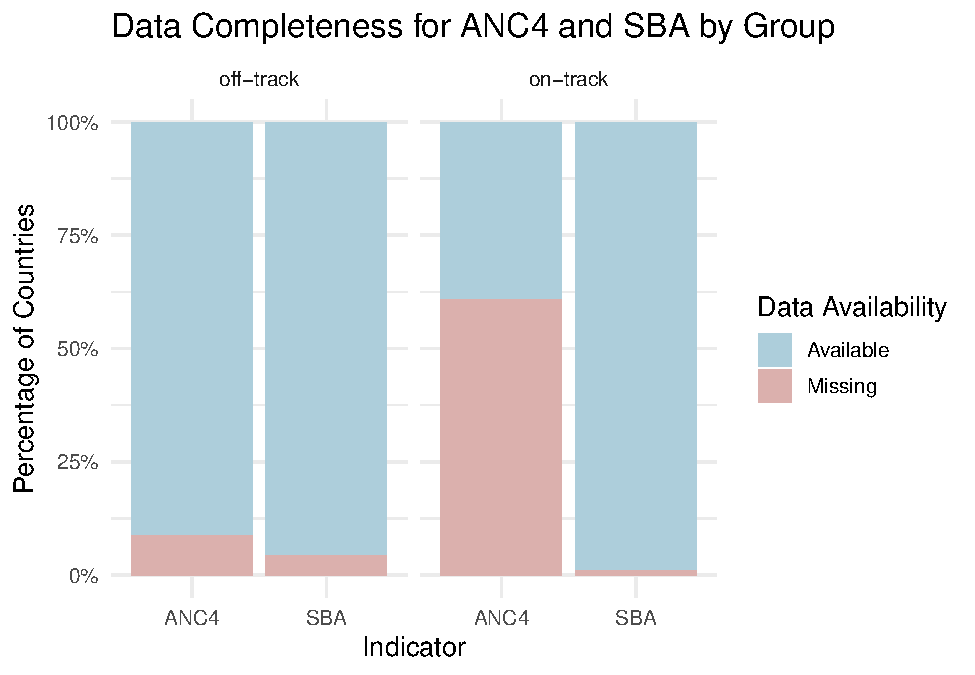
\includegraphics{/Users/luc_w/Documents/GitHub/unicef-coverage-analysis/04_output/01_report_output/03_report_files/figure-latex/data-completeness-stackedbar-1.pdf}

\textbf{Interpretation}\\
- Over 60\% of on-track countries lack ANC4 data, weakening group-level
reliability.\\
- SBA data is nearly complete, enabling stronger comparisons.\\
- \emph{27.4\%} of countries were fully excluded due to missing group,
births, or both indicators.\\
- Others were partially included, lacking ANC4 but contributing SBA data
--- highlighting antenatal reporting gaps.\\
- The table below outlines missing data patterns to guide data system
improvements.

\begin{longtable}[t]{lrr}
\caption{\label{tab:exclusion-summary-table}Missing data patterns}\\
\toprule
Exclusion Reason & \# Countries & Share (\%)\\
\midrule
Missing ANC4 only & 67 & 42.1\\
Missing ANC4 and SBA & 45 & 28.3\\
Missing U5MR group, ANC4, and SBA & 38 & 23.9\\
Missing SBA only & 4 & 2.5\\
Missing group & 4 & 2.5\\
\addlinespace
Missing U5MR group, ANC4, SBA, and births & 1 & 0.6\\
\bottomrule
\end{longtable}

\begin{center}\rule{0.5\linewidth}{0.5pt}\end{center}

\subsubsection{2.3 Country-Level coverage: interactive
view}\label{country-level-coverage-interactive-view}

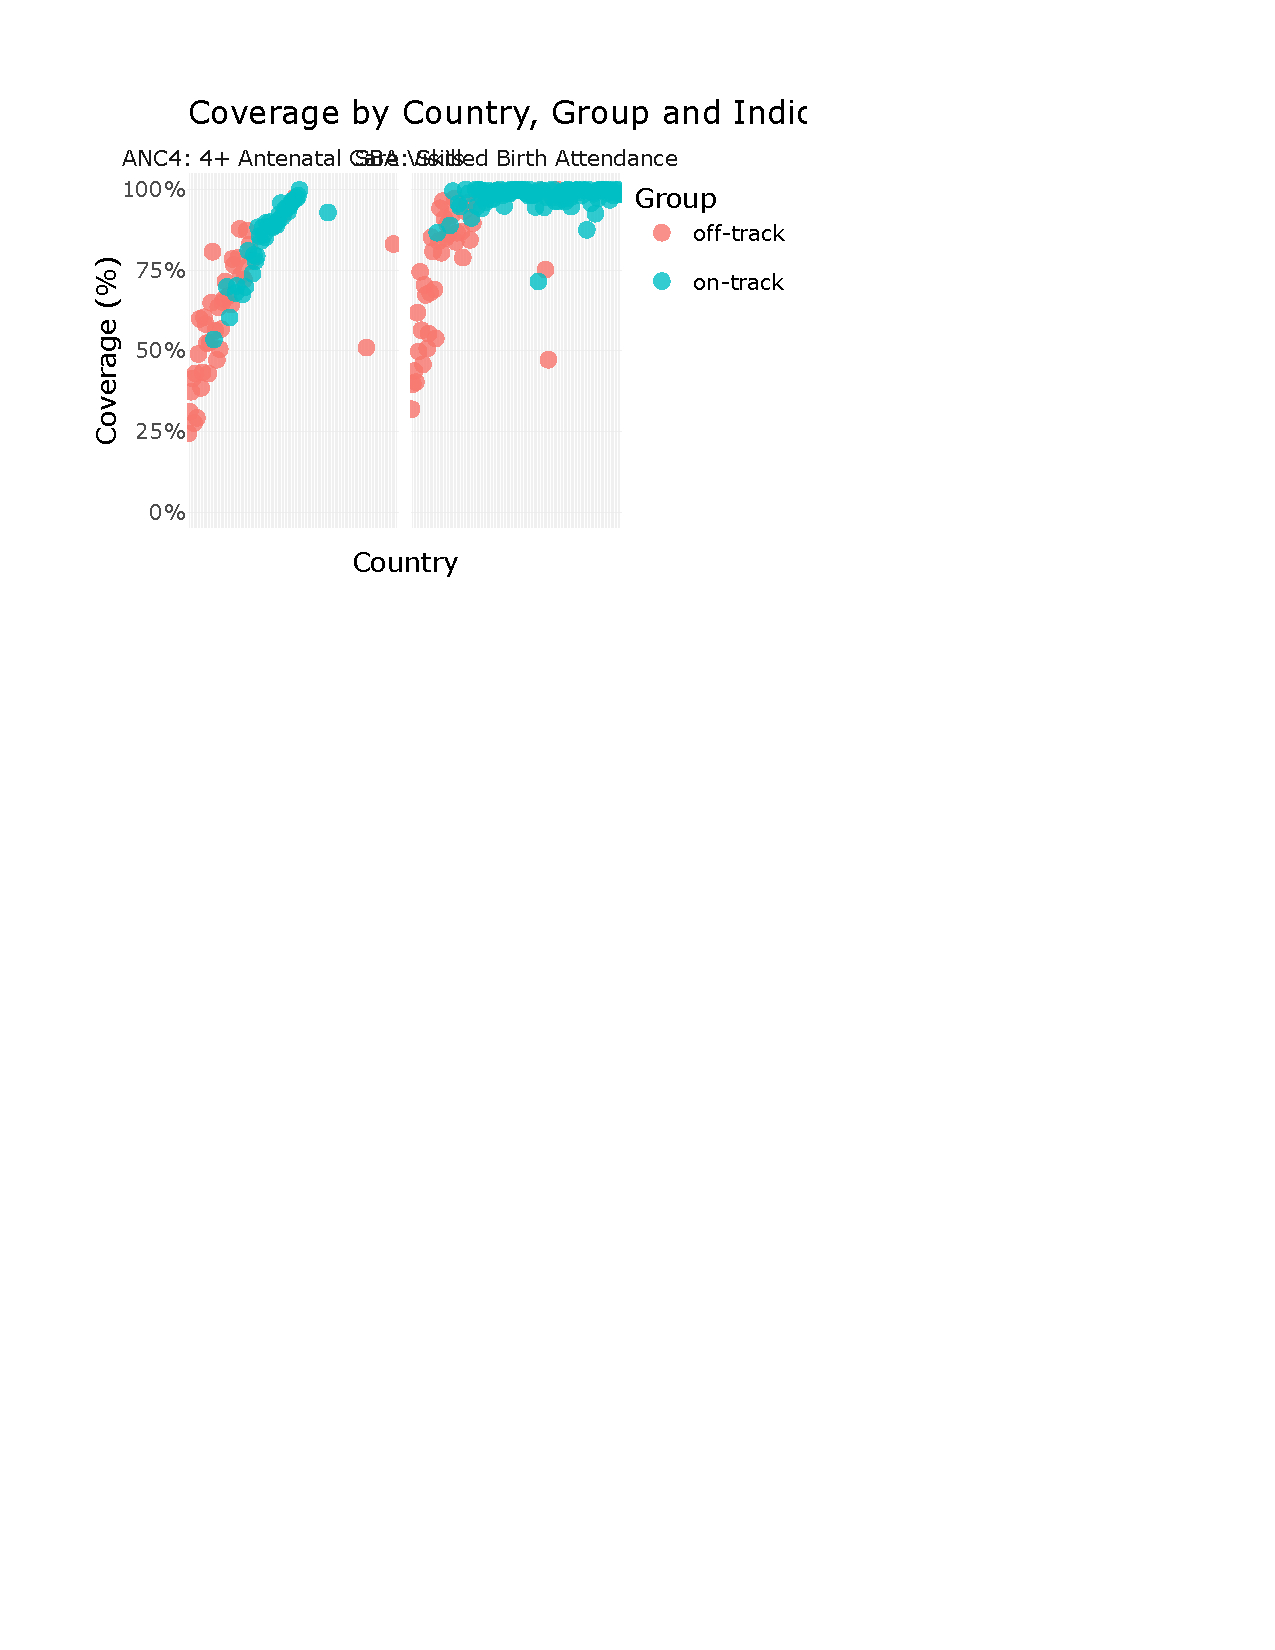
\includegraphics{/Users/luc_w/Documents/GitHub/unicef-coverage-analysis/04_output/01_report_output/03_report_files/figure-latex/unnamed-chunk-2-1.pdf}

\textbf{Interpretation}\\
This graph highlights the contrast between \textbf{ANC4} and
\textbf{SBA} coverage by country group:

\begin{itemize}
\tightlist
\item
  \textbf{SBA coverage} is consistently high, with most countries
  reaching or exceeding \textbf{80\%}.
\item
  \textbf{ANC4 coverage}, however, is more variable --- particularly in
  \emph{off-track} countries, where it often falls \textbf{below 60\%}.
\end{itemize}

➡️ \emph{See Section 2.4 for summary distributions.}

\begin{quote}
\textbf{Note}: Best viewed in HTML for tooltip interactivity.
\end{quote}

\begin{center}\rule{0.5\linewidth}{0.5pt}\end{center}

\subsubsection{2.4 Coverage distribution by
group}\label{coverage-distribution-by-group}

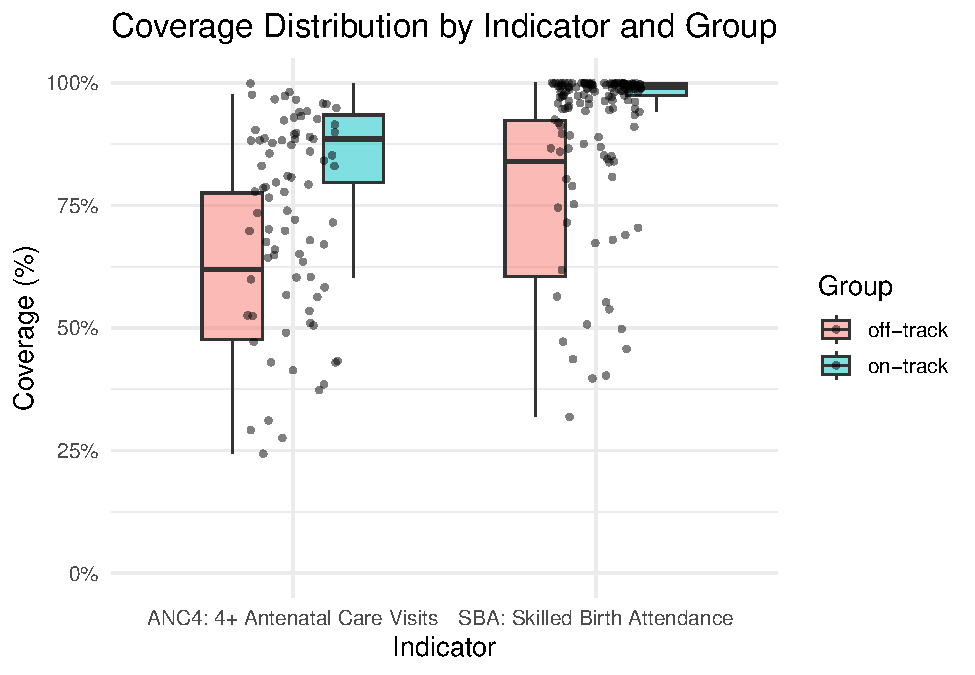
\includegraphics{/Users/luc_w/Documents/GitHub/unicef-coverage-analysis/04_output/01_report_output/03_report_files/figure-latex/unnamed-chunk-3-1.pdf}

\textbf{Interpretation}\\
This distribution plot shows the \textbf{range and central tendency} of
ANC4 and SBA coverage by country group. The \textbf{median SBA is high}
for both groups, while \textbf{ANC4 coverage is lower and more
dispersed}, especially in off-track settings. On-track countries appear
to perform slightly better in ANC4, but many are missing data, as noted
earlier.

The wider spread in ANC4 for off-track countries also highlights
\textbf{greater inequality in antenatal care access}, pointing to
\textbf{potential structural or systemic challenges} in reaching women
early in pregnancy.

\begin{center}\rule{0.5\linewidth}{0.5pt}\end{center}

\subsubsection{2.5 ANC4 vs SBA
Scatterplot}\label{anc4-vs-sba-scatterplot}

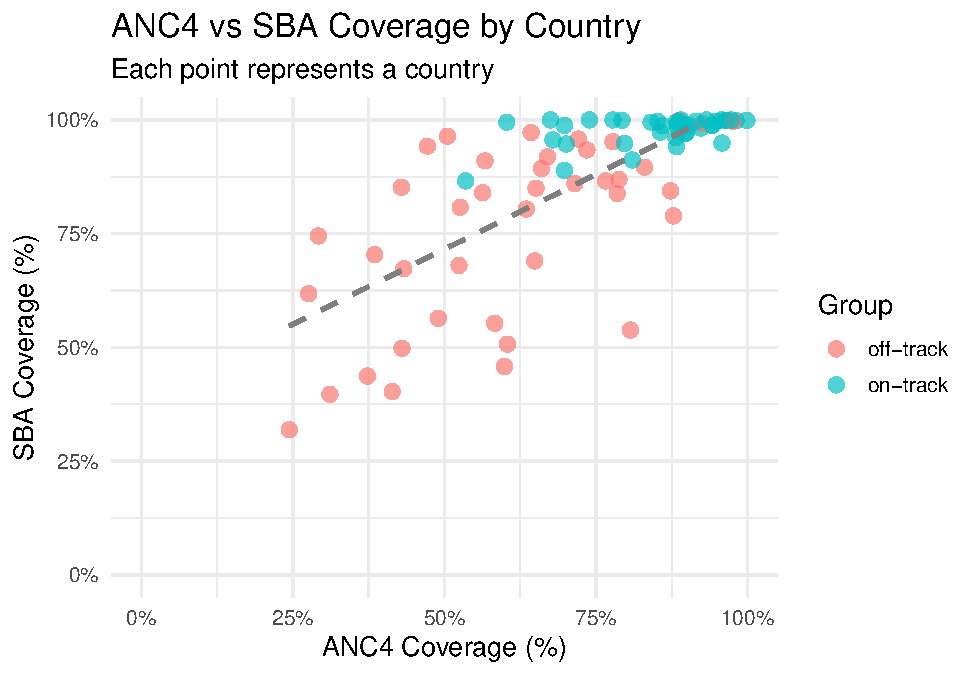
\includegraphics{/Users/luc_w/Documents/GitHub/unicef-coverage-analysis/04_output/01_report_output/03_report_files/figure-latex/scatter-anc4-sba-1.pdf}

\textbf{Interpretation}\\
This scatterplot highlights the relationship between ANC4 and SBA
coverage across countries. While many countries show a positive
correlation, a significant cluster of off-track countries exhibit high
SBA coverage but low ANC4, indicating that women are receiving delivery
care without adequate antenatal follow-up.

\begin{center}\rule{0.5\linewidth}{0.5pt}\end{center}

\begin{quote}
\textbf{Key Summary Insight (applies across Sections 2.1--2.5):}\\
\textbf{SBA coverage is consistently strong}, indicating widespread
access to delivery care. In contrast, \textbf{ANC4 coverage remains
limited or missing}, especially in off-track countries and many on-track
countries. This imbalance reveals critical gaps in early maternal
engagement and system continuity.
\end{quote}

\begin{center}\rule{0.5\linewidth}{0.5pt}\end{center}

\subsubsection{2.6 Countries with lowest ANC4
coverage}\label{countries-with-lowest-anc4-coverage}

\begin{longtable}[t]{llrr}
\caption{\label{tab:unnamed-chunk-4}Top 10 Countries with Lowest Combined ANC4 and SBA Coverage}\\
\toprule
Country & Group & ANC4 Coverage (\%) & SBA Coverage (\%)\\
\midrule
Somalia & off-track & 24.4 & 31.9\\
South Sudan & off-track & 31.1 & 39.7\\
Niger & off-track & 37.3 & 43.7\\
Central African Republic & off-track & 41.4 & 40.3\\
Afghanistan & off-track & 27.6 & 61.8\\
\addlinespace
Ethiopia & off-track & 43.0 & 49.8\\
Senegal & off-track & 29.2 & 74.5\\
Papua New Guinea & off-track & 49.0 & 56.4\\
Madagascar & off-track & 59.9 & 45.8\\
Mauritania & off-track & 38.5 & 70.4\\
\bottomrule
\end{longtable}

\begin{quote}
These countries face compounded vulnerabilities in both antenatal and
delivery services. Addressing gaps in the full maternal health continuum
is essential for reducing preventable maternal and neonatal deaths.
\end{quote}

\begin{center}\rule{0.5\linewidth}{0.5pt}\end{center}

\section{3. Interpretation}\label{interpretation}

The results highlights \textbf{strong skilled birth attendance (SBA)}
across all countries, but also reveals \textbf{significant challenges
with antenatal care coverage (ANC4)}, particularly in \textbf{off-track
countries} and in \textbf{on-track countries} where data is missing or
incomplete. This imbalance raises concerns about the \textbf{continuity
of maternal care}, a key element for achieving \textbf{SDG targets 3.1
and 3.2}.

\paragraph{\texorpdfstring{\textbf{Coverage comparison by country
group}}{Coverage comparison by country group}}\label{coverage-comparison-by-country-group}

\begin{longtable}[]{@{}
  >{\raggedright\arraybackslash}p{(\columnwidth - 4\tabcolsep) * \real{0.2778}}
  >{\raggedright\arraybackslash}p{(\columnwidth - 4\tabcolsep) * \real{0.3333}}
  >{\raggedright\arraybackslash}p{(\columnwidth - 4\tabcolsep) * \real{0.3889}}@{}}
\toprule\noalign{}
\begin{minipage}[b]{\linewidth}\raggedright
\textbf{Metric}
\end{minipage} & \begin{minipage}[b]{\linewidth}\raggedright
\textbf{On-Track Countries}
\end{minipage} & \begin{minipage}[b]{\linewidth}\raggedright
\textbf{Off-Track Countries}
\end{minipage} \\
\midrule\noalign{}
\endhead
\bottomrule\noalign{}
\endlastfoot
\textbf{SBA coverage} & High, with little variation & Also high and
relatively stable \\
\textbf{ANC4 coverage} & More heterogeneous & Often low, typically
\textless{} 60\% \\
\textbf{ANC4 data completeness} & Poor: \textasciitilde60\% of countries
missing & Good: Nearly all countries reported \\
\end{longtable}

\begin{quote}
These results suggest that while many women receive skilled support
during delivery, antenatal engagement remains limited in several
contexts --- either due to insufficient coverage or the absence of
reliable data.
\end{quote}

\subsubsection{\texorpdfstring{\textbf{Why is ANC4 Low or
Missing?}}{Why is ANC4 Low or Missing?}}\label{why-is-anc4-low-or-missing}

ANC4 is inherently \textbf{more difficult to capture and deliver} than
SBA. Unlike delivery, which is a single event often occurring in a
facility, ANC4 requires \textbf{multiple visits}, spread over months.
Several factors contribute to low uptake or missing data:

\begin{itemize}
\tightlist
\item
  \textbf{Economic barriers} (e.g., transport costs, informal fees)
\item
  \textbf{Time constraints} (especially for women with household or work
  responsibilities)
\item
  \textbf{Distance and infrastructure}
\item
  \textbf{Lack of awareness or trust in health systems}
\end{itemize}

\begin{quote}
In contrast, SBA, a one-time event, is easier to track and often better
integrated into health systems.
\end{quote}

Several of the \textbf{lowest-performing countries} , including
\emph{Somalia, South Sudan, Niger, Central African Republic}, and
\emph{Afghanistan} --- report \textbf{ANC4 and SBA coverage both below
50\%}. These countries represent \textbf{critical gaps in maternal care}
that affect both early and delivery-stage interventions. Others, such as
\emph{Senegal} and \emph{Mauritania}, show \textbf{moderate SBA coverage
but extremely low ANC4 uptake}, pointing to a \textbf{breakdown in
continuity of care} during pregnancy. All countries in this list are
\textbf{off-track} in under-five mortality, reinforcing the urgency of
targeted action.

\begin{center}\rule{0.5\linewidth}{0.5pt}\end{center}

\section{4 Strategic Recommendations}\label{strategic-recommendations}

\paragraph{\texorpdfstring{\textbf{For On-Track
Countries}}{For On-Track Countries}}\label{for-on-track-countries}

\begin{itemize}
\tightlist
\item
  \textbf{Close the ANC4 data gap}:

  \begin{itemize}
  \tightlist
  \item
    Improve antenatal data availability through routine health
    information systems and survey coverage.
  \item
    When unavailable, triangulate ANC4 estimates using facility,
    insurance, or digital health records.
  \end{itemize}
\item
  \textbf{Ensure quality beyond SBA}:

  \begin{itemize}
  \tightlist
  \item
    Validate success with maternal care: High SBA alone isn't
    sufficient. Without ANC4, risks remain high. Ensure ``on-track''
    status includes quality and continuity of care.
  \end{itemize}
\end{itemize}

\paragraph{\texorpdfstring{\textbf{For Off-Track
Countries}}{For Off-Track Countries}}\label{for-off-track-countries}

\begin{itemize}
\tightlist
\item
  \textbf{Invest in antenatal access}:

  \begin{itemize}
  \tightlist
  \item
    Address \textbf{geographic, economic, and sociocultural barriers} to
    early pregnancy care.\\
  \item
    Use \textbf{mobile clinics, community health workers}, and local
    outreach to reach underserved women.
  \item
    \emph{Note: Countries with both low ANC4 and SBA (e.g.,
    \textbf{Somalia}, \textbf{South Sudan}, \textbf{Niger},
    \textbf{CAR}) require foundational investment in access and
    coverage.}
  \end{itemize}
\item
  \textbf{Correct the care imbalance}:

  \begin{itemize}
  \tightlist
  \item
    In countries with high SBA but low ANC4 (e.g., \textbf{Senegal},
    \textbf{Mauritania}), encourage early pregnancy contact through
    targeted interventions and communication strategies.
  \end{itemize}
\end{itemize}

\paragraph{\texorpdfstring{\textbf{For All
Countries}}{For All Countries}}\label{for-all-countries}

\begin{itemize}
\tightlist
\item
  \textbf{Enhance equity and targeting}:

  \begin{itemize}
  \tightlist
  \item
    Disaggregate ANC4/SBA coverage by \textbf{age, location, wealth, and
    parity} to uncover hidden gaps.
  \end{itemize}
\item
  \textbf{Institutionalize annual monitoring}:

  \begin{itemize}
  \tightlist
  \item
    Align ANC4/SBA tracking with DHS/MICS cycles and integrate
    indicators into national dashboards.
  \end{itemize}
\item
  \textbf{Commission deeper research}

  \begin{itemize}
  \tightlist
  \item
    A \textbf{targeted study is needed} to understand low ANC4 uptake,
    combining \textbf{demand-side factors} (awareness, distance, cost)
    with \textbf{supply-side barriers} (health system reach, data gaps).
  \end{itemize}
\end{itemize}

\begin{center}\rule{0.5\linewidth}{0.5pt}\end{center}

\section{5. Sources}\label{sources}

\begin{itemize}
\tightlist
\item
  WHO Indicator Metadata:

  \begin{itemize}
  \tightlist
  \item
    \href{https://www.who.int/data/gho/indicator-metadata-registry/imr-details/80}{ANC4}
  \item
    \href{https://data.who.int/indicators/i/F835E3B/1772666}{SBA}
  \end{itemize}
\item
  \href{https://data.unicef.org/topic/child-survival/under-five-mortality/}{UNICEF
  Under-Five Mortality (U5MR) Overview} -- used to define on-track and
  off-track country groupings.
\item
  UN SDG Indicator Metadata:

  \begin{itemize}
  \tightlist
  \item
    \href{https://unstats.un.org/sdgs/metadata/files/Metadata-03-01-01.pdf}{SDG
    3.1.1 -- Maternal Mortality}
  \item
    \href{https://unstats.un.org/sdgs/metadata/files/Metadata-03-01-02.pdf}{SDG
    3.1.2 -- Skilled Birth Attendance (SBA)}
  \item
    \href{https://unstats.un.org/sdgs/metadata/files/Metadata-03-02-01.pdf}{SDG
    3.2.1 -- Under-Five Mortality}
  \item
    \href{https://unstats.un.org/sdgs/metadata/files/Metadata-03-02-02.pdf}{SDG
    3.2.2 -- Neonatal Mortality}
  \end{itemize}
\item
  Data derived from analytical script \texttt{02\_analysis.R}
  (consultancy assessment deliverable)
\end{itemize}

\end{document}
